% !TEX encoding = UTF-8
% !TEX program = lualatex
% !TEX spellcheck = zh_CN
\documentclass[10pt,aspectratio=169,english]{beamer}
%%%%%%%%%%%%%%%%%% 引入配置文件 %%%%%%%%%%%%%%%%%%
\usepackage{ctex}
\usepackage{hologo}
\usepackage{luamesh}
\usepackage{booktabs}
\usepackage{makecell}
\usepackage{longtable}
\usepackage[table,xcdraw]{xcolor}
\usepackage{pgfpages}
\usepackage[most]{tcolorbox}
\usepackage{graphics}
\usepackage{subcaption}
\usepackage{float}
\usepackage{listings}
\usepackage[linesnumbered,commentsnumbered,ruled,lined]{algorithm2e} 
\usepackage{multirow}
\usepackage[sort,numbers]{natbib}
 % 宏包
\newcommand{\bbR}{\mathbb{R}} % mathbb{R}
\newcommand{\tr}{\mathrm{tr}} % 定义迹符号
\newcommand{\T}{^\mathrm{T}} % 转置符号
\newcommand{\norm}[1]{\left\Vert{#1}\right\Vert} % 定义范数符号
\newcommand{\rank}{\mathrm{rank}} % 定义秩符号
\newcommand{\subjectto}{\mathrm{s.t.\quad}} % 定义 s.t. 符号
\newcommand{\KL}{\mathrm{KL}} % 定义 KL 符号
\newcommand{\N}{\mathcal{N}} % 定义 N 符号
\newcommand{\E}{\mathbb{E}} % 定义期望符号
\newcommand{\ELBO}{\mathrm{ELBO}} % 定义ELBO符号
\newcommand{\Cov}{\mathrm{Cov}} % 定义协方差符号
\newcommand{\decoder}{\mathrm{dec}} % 定义 decoder
\newcommand{\iidsim}{\overset{\text{iid}}{\sim}} % 定义 iid


% 微分符号
\newcommand{\rmd}{\mathrm{d}} % 定义整体微分d
\newcommand{\dx}{\mathrm{d}x} % dx
\newcommand{\dxb}{\mathrm{d}\boldsymbol{x}} % dxb
\newcommand{\dzb}{\mathrm{d}\boldsymbol{z}} % dzb

% 积分符号
\newcommand{\displayint}{\displaystyle\int\nolimits} % 定义整体微分d

% 矢量符号
\newcommand{\rb}{\boldsymbol{r}} % rb
\newcommand{\zeros}{\boldsymbol{0}} % zeros
\newcommand{\Ib}{\boldsymbol{\mathrm{I}}} % Ib
\newcommand{\yb}{\boldsymbol{y}} % yb
\newcommand{\xb}{\boldsymbol{x}} % xb
\newcommand{\Xb}{\boldsymbol{X}} % Xb
\newcommand{\Rb}{\boldsymbol{R}} % Rb
\newcommand{\zb}{\boldsymbol{z}} % zb
\newcommand{\thetab}{\boldsymbol{\theta}} % thetab
\newcommand{\phib}{\boldsymbol{\phi}} % phi
\newcommand{\epsilonb}{\boldsymbol{\epsilon}} % epsilonb
\newcommand{\mub}{\boldsymbol{\mu}} % mub
\newcommand{\Sigmab}{\boldsymbol{\Sigma}} % Sigmab
 % 自定义命令
%%%%%%%%%%%%%%%%%%%%%%%%%%%%%%% Remark %%%%%%%%%%%%%%%%%%%%%%%%%%%%%%%
\definecolor{Remarkcolframe}{RGB}{0,110,184}
\makeatletter
\newtcbtheorem[number within=section]{beamerremark}{Remark}{
	enhanced,
	before skip=2mm,
	after skip=2mm,
	breakable,
	colframe=Remarkcolframe,
	colback=Remarkcolframe!4!white,
	boxrule=1.5pt,
	attach boxed title to top left={xshift=1cm,yshift*=1mm-\tcboxedtitleheight},
	fonttitle=\bfseries,
	boxed title style={frame code={
			\path[fill=Remarkcolframe]
			([yshift=-1mm,xshift=-1mm]frame.north west)
			arc[start angle=0,end angle=180,radius=1mm]
			([yshift=-1mm,xshift=1mm]frame.north east)
			arc[start angle=180,end angle=0,radius=1mm];
			\path[left color=Remarkcolframe,right color=Remarkcolframe,
			middle color=Remarkcolframe]
			([xshift=-2mm]frame.north west) -- ([xshift=2mm]frame.north east)
			[rounded corners=1mm]-- ([xshift=1mm,yshift=-1mm]frame.north east)
			-- (frame.south east) -- (frame.south west)
			-- ([xshift=-1mm,yshift=-1mm]frame.north west)
			[sharp corners]-- cycle;
		},interior engine=empty,
	},
	#1
}{rmk} % 引用标签
\makeatother




%%%%%%%%%%%%%%%%%%%%%%%%%%%%%%% Question %%%%%%%%%%%%%%%%%%%%%%%%%%%%%%%
\definecolor{Questioncolframe}{HTML}{3d7463}
\makeatletter
\newtcbtheorem[number within=section]{beamerquestion}{Question}{
	enhanced,
	breakable, 
	colframe=Questioncolframe,
	colback=Questioncolframe!4!white,
	attach boxed title to top left={yshift*=-\tcboxedtitleheight},
	fonttitle=\bfseries,
	boxed title size=title,
	boxed title style={%
		sharp corners,
		rounded corners=northwest,
		colback=tcbcolframe,
		boxrule=0pt,
	},
	underlay boxed title={%
		\path[fill=tcbcolframe] (title.south west)--(title.south east)
		to[out=0, in=180] ([xshift=5mm]title.east)--
		(title.center-|frame.east)
		[rounded corners=\kvtcb@arc] |-
		(frame.north) -| cycle;
	},
	#1
}{qs} % 引用标签
\makeatother




%%%%%%%%%%%%%%%%%%%%%%%%%%%%%%% Definition %%%%%%%%%%%%%%%%%%%%%%%%%%%%%%%
\definecolor{Definitioncolframe}{HTML}{2b8da3}
\makeatletter
\newtcbtheorem[number within=section]{beamerdefinition}{Definition}{
	shadow={1mm}{-1mm}{0mm}{black!15!white}, % 阴影
	parbox=false, % 添加缩进
	enhanced,
	breakable,
	colframe = Definitioncolframe,
	colback = Definitioncolframe!4!white,
	coltitle = Definitioncolframe,
	frame hidden,
	borderline west = {3pt}{0pt}{Definitioncolframe},
	fonttitle=\bfseries,
	boxrule = 0pt,
	sharp corners,
	detach title,
	before upper = \tcbtitle\par\smallskip,
	segmentation style={solid, Definitioncolframe},
	#1
}{dfn} % 引用标签
\makeatother




%%%%%%%%%%%%%%%%%%%%%%%%%%%%%%% Property %%%%%%%%%%%%%%%%%%%%%%%%%%%%%%%
\definecolor{Propertycolframe}{HTML}{0c3d92}
\makeatletter
\newtcbtheorem[number within=section]{beamerproperty}{Property}{
	shadow={1mm}{-1mm}{0mm}{black!15!white}, % 阴影
	parbox=false, % 添加缩进
	enhanced,
	breakable,
	colframe = Propertycolframe,
	colback = Propertycolframe!4!white,
	coltitle = Propertycolframe,
	frame hidden,
	borderline west = {3pt}{0pt}{Propertycolframe},
	fonttitle=\bfseries,
	boxrule = 0pt,
	sharp corners,
	detach title,
	before upper = \tcbtitle\par\smallskip,
	segmentation style={solid, Propertycolframe},
	#1
}{pro} % 引用标签
\makeatother




%%%%%%%%%%%%%%%%%%%%%%%%%%%%%%% Example %%%%%%%%%%%%%%%%%%%%%%%%%%%%%%%
\definecolor{Examplecolframe}{HTML}{a4d65e}
\makeatletter
\newtcbtheorem[number within=section]{beamerexample}{Example}{
	parbox=false, % 添加缩进
	shadow={1mm}{-1mm}{0mm}{black!15!white}, % 阴影
	enhanced,
	breakable,
	colframe = Examplecolframe,
	colback = Examplecolframe!4!white,
	coltitle = Examplecolframe,
	fonttitle = \bfseries,
	boxrule = 1.5pt,
	sharp corners,
	detach title,
	before upper = \tcbtitle\par\smallskip,
	segmentation style={solid, Examplecolframe},
	#1
}{ex} % 引用标签
\makeatother




%%%%%%%%%%%%%%%%%%%%%%%%%%%%%%% Theorem %%%%%%%%%%%%%%%%%%%%%%%%%%%%%%%
\definecolor{Theoremcolframe}{HTML}{f3722c}
\makeatletter
\newtcbtheorem[number within=section]{beamertheorem}{Theorem}{
	parbox=false, % 添加缩进
	shadow={1mm}{-1mm}{0mm}{black!15!white}, % 阴影
	enhanced,
	breakable,
	colframe = Theoremcolframe,
	colback = Theoremcolframe!4!white,
	coltitle = Theoremcolframe,
	frame hidden,
	borderline west = {3pt}{0pt}{Theoremcolframe},
	fonttitle = \bfseries,
	boxrule = 0pt,
	sharp corners,
	detach title,
	before upper = \tcbtitle\par\smallskip,
	segmentation style={solid, Theoremcolframe},
	#1
}{thm} % 引用标签
\makeatother




%%%%%%%%%%%%%%%%%%%%%%%%%%%%%%% Corollary %%%%%%%%%%%%%%%%%%%%%%%%%%%%%%%
\definecolor{Corollarycolframe}{HTML}{ff4d94}
\makeatletter
\newtcbtheorem[number within=section]{beamercorollary}{Corollary}{
	parbox=false, % 添加缩进
	shadow={1mm}{-1mm}{0mm}{black!15!white}, % 阴影
	enhanced,
	breakable,
	colframe = Corollarycolframe,
	colback = Corollarycolframe!4!white,
	coltitle = Corollarycolframe,
	frame hidden,
	borderline west = {3pt}{0pt}{Corollarycolframe},
	fonttitle = \bfseries,
	boxrule = 0sp,
	sharp corners,
	detach title,
	before upper = \tcbtitle\par\smallskip,
	segmentation style={solid, Corollarycolframe},
	#1
}{cor} % 引用标签
\makeatother




%%%%%%%%%%%%%%%%%%%%%%%%%%%%%%% Lemma %%%%%%%%%%%%%%%%%%%%%%%%%%%%%%%
\definecolor{Lemmacolframe}{HTML}{d72948}
\makeatletter
\newtcbtheorem[number within=section]{beamerlemma}{Lemma}{
	parbox=false, % 添加缩进
	shadow={1mm}{-1mm}{0mm}{black!15!white}, % 阴影
	enhanced,
	breakable,
	colframe = Lemmacolframe,
	colback = Lemmacolframe!4!white,
	coltitle = Lemmacolframe,
	frame hidden,
	borderline west = {3pt}{0pt}{Lemmacolframe},
	fonttitle = \bfseries,
	boxrule = 0sp,
	sharp corners,
	detach title,
	before upper = \tcbtitle\par\smallskip,
	segmentation style={solid, Lemmacolframe},
	#1
}{lm} % 引用标签
\makeatother




%%%%%%%%%%%%%%%%%%%%%%%%%%%%%%% Proposition %%%%%%%%%%%%%%%%%%%%%%%%%%%%%%%
\definecolor{Propositioncolframe}{HTML}{b56fbf}
\makeatletter
\newtcbtheorem[number within=section]{beamerproposition}{Proposition}{
	parbox=false, % 添加缩进
	shadow={1mm}{-1mm}{0mm}{black!15!white}, % 阴影
	enhanced,
	breakable,
	colframe = Propositioncolframe,
	colback = Propositioncolframe!4!white,
	coltitle = Propositioncolframe,
	frame hidden,
	borderline west = {3pt}{0pt}{Propositioncolframe},
	fonttitle = \bfseries,
	boxrule = 0sp,
	sharp corners,
	detach title,
	before upper = \tcbtitle\par\smallskip,
	segmentation style={solid, Propositioncolframe},
	#1
}{prp} % 引用标签
\makeatother



%%%%%%%%%%%%%%%%%%%%%%%%%%%%%%% Solution %%%%%%%%%%%%%%%%%%%%%%%%%%%%%%%
\definecolor{solutioncol}{HTML}{007B8A}
\newcommand{\beamersolution}{\textbf{\color{solutioncol}{Solution. }}}



%%%%%%%%%%%%%%%%%%%%%%%%%%%%%%% Proof %%%%%%%%%%%%%%%%%%%%%%%%%%%%%%%
\definecolor{Proofcol}{HTML}{4dd0e1}
\renewcommand{\proofname}{\rm \textcolor{Proofcol}{\bfseries Proof.}}





 % 自定义数学样式
%%%%%%%%%%%%%%%%%% 文档临时设置 %%%%%%%%%%%%%%%%%%
\usetheme[
amurmapleblue, % 主题颜色
delaunay, % 开启网格背景
nomail, % 取消左侧邮箱
% nogauge, % 取消左侧进度条
]{Amurmaple}
\usefonttheme{serif} % 字体主题为衬线字体
\setbeamertemplate{caption}[numbered] % 启用 figure 和 table 编号
\numberwithin{equation}{section}  % 公式编号 (section.number) 格式

\lstdefinestyle{liststyle}{
	basicstyle=\ttfamily\scriptsize,
	keywordstyle=\color{AmurmapleBlue}\bfseries,
	commentstyle=\color{gray},
	stringstyle=\color{AmurmapleOrange},
	breaklines=true,
	breakatwhitespace=true,
	columns=fullflexible,
	keepspaces=true,
	frame=single,
	framerule=0.4pt,
	rulecolor=\color{black!20},
	backgroundcolor=\color{black!2},
	xleftmargin=0.5em,
	xrightmargin=0.5em,
}
\lstset{style=liststyle,language=[LaTeX]TeX}

%%%%%%%%%%%%%%%%%% document %%%%%%%%%%%%%%%%%%

% 封面页信息
% logo
\titlegraphic{
\includegraphics[width=3.38cm]{./Figures/Logos/USTC_logo_blue.pdf}}
% 基本信息
\author[USTC]{\Large{USTC Amurmaple}}
\mail{zhiyuanjiaustc2025@mail.ustc.edu.cn}
\webpage{https://www.ustc.edu.cn/}
\institute{环境科学与光电技术学院}
\date{\today}
\title[USTC Amurmaple 文档]{
	\centering\Huge{USTC Amurmaple Document}
}
\subtitle{Beamer 模板使用手册}
\collaboration{\large\textbf{基于 Beamer、\LaTeX{} 与 Amurmaple 主题}}

%% logo
\titlegraphic{
\includegraphics[width=3.38cm]{./Figures/Logos/USTC_logo_blue.pdf}}
% 基本信息
\author[Sidebar Author]{\Large{Title Page Author}}
\mail{Your mail}
\webpage{Your Webpage}
\institute{Your Institute}
\date{Reporting Date}
\title[Sidebar Title]{\centering\Huge{The Title of Your Beamer}}
\subtitle{Your Beamer Subtitle}
\collaboration{\large\textbf{Your Collaboration Information}}





\begin{document}
	% TitlePage
	\maketitle
	
	% Contents
	\sepframe[
title={目录 Contents},
image={
\includegraphics[width=9cm]{./Figures/Logos/USTC_slide_blue.pdf}}
]

	
	% Sections
	\section{模板简介}
%\sepframe[image={
\includegraphics[width=3.38cm]{./Figures/Logos/USTC_logo_blue.pdf}}]
% \sepframe 无插入 logo 的分隔页
\sepframe[image={
\includegraphics[width=3.38cm]{./Figures/Logos/USTC_logo_blue.pdf}}]

\begin{frame}{模板定位}
	\begin{information}[USTC Amurmaple 简介]
		本模板是在 Amurmaple Beamer Theme 及众多二次开发者的基础上，为中国科学技术大学报告场景整理的演示文稿模板。项目已经将主题、宏包、自定义命令、正文分节和参考文献拆分到不同目录，适合用于课程汇报、组会报告、开题答辩和阶段性科研展示。
	\end{information}
	
	\begin{block}{项目入口}
		\begin{itemize}
			\item 写作从 \texttt{main.tex} 开始；
			\item 使用 \hologo{LuaLaTeX} 编译。
		\end{itemize}
	\end{block}
\end{frame}



\begin{frame}{项目结构}
\begin{minipage}[t]{\linewidth}
\texttt{
	\begin{block}{核心文件}
		\begin{itemize}
			\item main.tex：演示文稿入口文件
			\item beamerthemeAmurmaple.sty：主题样式
		\end{itemize}
	\end{block}
}
\end{minipage}

\vspace*{1em}
\begin{minipage}[t]{0.5\linewidth}
	\texttt{
		\begin{block}{文件夹介绍 I}
			\begin{itemize}
				% Bibliography
				\item Bibliography
				\begin{itemize}
					\item Bibliography.tex：被引入 main.tex
					\item gbt7714-numerical.bst：.bst 格式文件
					\item MyBibliography.bib：BibTeX 数据库
				\end{itemize}
				% Configure
				\item Configure
				\begin{itemize}
					\item beamerMathStyle.tex：自定义数学样式
					\item commands.tex：自定义命令
					\item packages.tex：宏包
				\end{itemize}
			\end{itemize}
		\end{block}
	}
\end{minipage}\hspace*{1em}
\begin{minipage}[t]{0.45\linewidth}
	\texttt{
		\begin{block}{文件夹介绍 II}
			\begin{itemize}
				% Figures
				\item Figures
				\begin{itemize}
					\item Logos：USTC 相关 logo
					\item 其他：所需要的图片
				\end{itemize}
				% Sections
				\item Sections
				\begin{itemize}
					\item TitlePageInformation.tex：封面页
					\item Content.tex：目录
					\item SectionX.tex：Section 内容
				\end{itemize}
			\end{itemize}
		\end{block}
	}
\end{minipage}
\end{frame}

	\section{快速开始}
%\sepframe[image={
\includegraphics[width=3.38cm]{./Figures/Logos/USTC_logo_blue.pdf}}]
% \sepframe 无插入 logo 的分隔页
\sepframe[image={
\includegraphics[width=3.38cm]{./Figures/Logos/USTC_logo_blue.pdf}}]

\begin{frame}[fragile]{推荐的项目入口 \texttt{main.tex}}

\begin{lstlisting}
% !TEX encoding = UTF-8
% !TEX program = lualatex
% !TEX spellcheck = zh_CN
\documentclass[10pt, aspectratio=169, english]{beamer}
\usepackage{ctex}
\usepackage{hologo}
\usepackage{luamesh}
\usepackage{booktabs}
\usepackage{makecell}
\usepackage{longtable}
\usepackage[table,xcdraw]{xcolor}
\usepackage{pgfpages}
\usepackage[most]{tcolorbox}
\usepackage{graphics}
\usepackage{subcaption}
\usepackage{float}
\usepackage{listings}
\usepackage[linesnumbered,commentsnumbered,ruled,lined]{algorithm2e} 
\usepackage{multirow}
\usepackage[sort,numbers]{natbib}
 % 宏包
\newcommand{\bbR}{\mathbb{R}} % mathbb{R}
\newcommand{\tr}{\mathrm{tr}} % 定义迹符号
\newcommand{\T}{^\mathrm{T}} % 转置符号
\newcommand{\norm}[1]{\left\Vert{#1}\right\Vert} % 定义范数符号
\newcommand{\rank}{\mathrm{rank}} % 定义秩符号
\newcommand{\subjectto}{\mathrm{s.t.\quad}} % 定义 s.t. 符号
\newcommand{\KL}{\mathrm{KL}} % 定义 KL 符号
\newcommand{\N}{\mathcal{N}} % 定义 N 符号
\newcommand{\E}{\mathbb{E}} % 定义期望符号
\newcommand{\ELBO}{\mathrm{ELBO}} % 定义ELBO符号
\newcommand{\Cov}{\mathrm{Cov}} % 定义协方差符号
\newcommand{\decoder}{\mathrm{dec}} % 定义 decoder
\newcommand{\iidsim}{\overset{\text{iid}}{\sim}} % 定义 iid


% 微分符号
\newcommand{\rmd}{\mathrm{d}} % 定义整体微分d
\newcommand{\dx}{\mathrm{d}x} % dx
\newcommand{\dxb}{\mathrm{d}\boldsymbol{x}} % dxb
\newcommand{\dzb}{\mathrm{d}\boldsymbol{z}} % dzb

% 积分符号
\newcommand{\displayint}{\displaystyle\int\nolimits} % 定义整体微分d

% 矢量符号
\newcommand{\rb}{\boldsymbol{r}} % rb
\newcommand{\zeros}{\boldsymbol{0}} % zeros
\newcommand{\Ib}{\boldsymbol{\mathrm{I}}} % Ib
\newcommand{\yb}{\boldsymbol{y}} % yb
\newcommand{\xb}{\boldsymbol{x}} % xb
\newcommand{\Xb}{\boldsymbol{X}} % Xb
\newcommand{\Rb}{\boldsymbol{R}} % Rb
\newcommand{\zb}{\boldsymbol{z}} % zb
\newcommand{\thetab}{\boldsymbol{\theta}} % thetab
\newcommand{\phib}{\boldsymbol{\phi}} % phi
\newcommand{\epsilonb}{\boldsymbol{\epsilon}} % epsilonb
\newcommand{\mub}{\boldsymbol{\mu}} % mub
\newcommand{\Sigmab}{\boldsymbol{\Sigma}} % Sigmab
 % 自定义命令
%%%%%%%%%%%%%%%%%%%%%%%%%%%%%%% Remark %%%%%%%%%%%%%%%%%%%%%%%%%%%%%%%
\definecolor{Remarkcolframe}{RGB}{0,110,184}
\makeatletter
\newtcbtheorem[number within=section]{beamerremark}{Remark}{
	enhanced,
	before skip=2mm,
	after skip=2mm,
	breakable,
	colframe=Remarkcolframe,
	colback=Remarkcolframe!4!white,
	boxrule=1.5pt,
	attach boxed title to top left={xshift=1cm,yshift*=1mm-\tcboxedtitleheight},
	fonttitle=\bfseries,
	boxed title style={frame code={
			\path[fill=Remarkcolframe]
			([yshift=-1mm,xshift=-1mm]frame.north west)
			arc[start angle=0,end angle=180,radius=1mm]
			([yshift=-1mm,xshift=1mm]frame.north east)
			arc[start angle=180,end angle=0,radius=1mm];
			\path[left color=Remarkcolframe,right color=Remarkcolframe,
			middle color=Remarkcolframe]
			([xshift=-2mm]frame.north west) -- ([xshift=2mm]frame.north east)
			[rounded corners=1mm]-- ([xshift=1mm,yshift=-1mm]frame.north east)
			-- (frame.south east) -- (frame.south west)
			-- ([xshift=-1mm,yshift=-1mm]frame.north west)
			[sharp corners]-- cycle;
		},interior engine=empty,
	},
	#1
}{rmk} % 引用标签
\makeatother




%%%%%%%%%%%%%%%%%%%%%%%%%%%%%%% Question %%%%%%%%%%%%%%%%%%%%%%%%%%%%%%%
\definecolor{Questioncolframe}{HTML}{3d7463}
\makeatletter
\newtcbtheorem[number within=section]{beamerquestion}{Question}{
	enhanced,
	breakable, 
	colframe=Questioncolframe,
	colback=Questioncolframe!4!white,
	attach boxed title to top left={yshift*=-\tcboxedtitleheight},
	fonttitle=\bfseries,
	boxed title size=title,
	boxed title style={%
		sharp corners,
		rounded corners=northwest,
		colback=tcbcolframe,
		boxrule=0pt,
	},
	underlay boxed title={%
		\path[fill=tcbcolframe] (title.south west)--(title.south east)
		to[out=0, in=180] ([xshift=5mm]title.east)--
		(title.center-|frame.east)
		[rounded corners=\kvtcb@arc] |-
		(frame.north) -| cycle;
	},
	#1
}{qs} % 引用标签
\makeatother




%%%%%%%%%%%%%%%%%%%%%%%%%%%%%%% Definition %%%%%%%%%%%%%%%%%%%%%%%%%%%%%%%
\definecolor{Definitioncolframe}{HTML}{2b8da3}
\makeatletter
\newtcbtheorem[number within=section]{beamerdefinition}{Definition}{
	shadow={1mm}{-1mm}{0mm}{black!15!white}, % 阴影
	parbox=false, % 添加缩进
	enhanced,
	breakable,
	colframe = Definitioncolframe,
	colback = Definitioncolframe!4!white,
	coltitle = Definitioncolframe,
	frame hidden,
	borderline west = {3pt}{0pt}{Definitioncolframe},
	fonttitle=\bfseries,
	boxrule = 0pt,
	sharp corners,
	detach title,
	before upper = \tcbtitle\par\smallskip,
	segmentation style={solid, Definitioncolframe},
	#1
}{dfn} % 引用标签
\makeatother




%%%%%%%%%%%%%%%%%%%%%%%%%%%%%%% Property %%%%%%%%%%%%%%%%%%%%%%%%%%%%%%%
\definecolor{Propertycolframe}{HTML}{0c3d92}
\makeatletter
\newtcbtheorem[number within=section]{beamerproperty}{Property}{
	shadow={1mm}{-1mm}{0mm}{black!15!white}, % 阴影
	parbox=false, % 添加缩进
	enhanced,
	breakable,
	colframe = Propertycolframe,
	colback = Propertycolframe!4!white,
	coltitle = Propertycolframe,
	frame hidden,
	borderline west = {3pt}{0pt}{Propertycolframe},
	fonttitle=\bfseries,
	boxrule = 0pt,
	sharp corners,
	detach title,
	before upper = \tcbtitle\par\smallskip,
	segmentation style={solid, Propertycolframe},
	#1
}{pro} % 引用标签
\makeatother




%%%%%%%%%%%%%%%%%%%%%%%%%%%%%%% Example %%%%%%%%%%%%%%%%%%%%%%%%%%%%%%%
\definecolor{Examplecolframe}{HTML}{a4d65e}
\makeatletter
\newtcbtheorem[number within=section]{beamerexample}{Example}{
	parbox=false, % 添加缩进
	shadow={1mm}{-1mm}{0mm}{black!15!white}, % 阴影
	enhanced,
	breakable,
	colframe = Examplecolframe,
	colback = Examplecolframe!4!white,
	coltitle = Examplecolframe,
	fonttitle = \bfseries,
	boxrule = 1.5pt,
	sharp corners,
	detach title,
	before upper = \tcbtitle\par\smallskip,
	segmentation style={solid, Examplecolframe},
	#1
}{ex} % 引用标签
\makeatother




%%%%%%%%%%%%%%%%%%%%%%%%%%%%%%% Theorem %%%%%%%%%%%%%%%%%%%%%%%%%%%%%%%
\definecolor{Theoremcolframe}{HTML}{f3722c}
\makeatletter
\newtcbtheorem[number within=section]{beamertheorem}{Theorem}{
	parbox=false, % 添加缩进
	shadow={1mm}{-1mm}{0mm}{black!15!white}, % 阴影
	enhanced,
	breakable,
	colframe = Theoremcolframe,
	colback = Theoremcolframe!4!white,
	coltitle = Theoremcolframe,
	frame hidden,
	borderline west = {3pt}{0pt}{Theoremcolframe},
	fonttitle = \bfseries,
	boxrule = 0pt,
	sharp corners,
	detach title,
	before upper = \tcbtitle\par\smallskip,
	segmentation style={solid, Theoremcolframe},
	#1
}{thm} % 引用标签
\makeatother




%%%%%%%%%%%%%%%%%%%%%%%%%%%%%%% Corollary %%%%%%%%%%%%%%%%%%%%%%%%%%%%%%%
\definecolor{Corollarycolframe}{HTML}{ff4d94}
\makeatletter
\newtcbtheorem[number within=section]{beamercorollary}{Corollary}{
	parbox=false, % 添加缩进
	shadow={1mm}{-1mm}{0mm}{black!15!white}, % 阴影
	enhanced,
	breakable,
	colframe = Corollarycolframe,
	colback = Corollarycolframe!4!white,
	coltitle = Corollarycolframe,
	frame hidden,
	borderline west = {3pt}{0pt}{Corollarycolframe},
	fonttitle = \bfseries,
	boxrule = 0sp,
	sharp corners,
	detach title,
	before upper = \tcbtitle\par\smallskip,
	segmentation style={solid, Corollarycolframe},
	#1
}{cor} % 引用标签
\makeatother




%%%%%%%%%%%%%%%%%%%%%%%%%%%%%%% Lemma %%%%%%%%%%%%%%%%%%%%%%%%%%%%%%%
\definecolor{Lemmacolframe}{HTML}{d72948}
\makeatletter
\newtcbtheorem[number within=section]{beamerlemma}{Lemma}{
	parbox=false, % 添加缩进
	shadow={1mm}{-1mm}{0mm}{black!15!white}, % 阴影
	enhanced,
	breakable,
	colframe = Lemmacolframe,
	colback = Lemmacolframe!4!white,
	coltitle = Lemmacolframe,
	frame hidden,
	borderline west = {3pt}{0pt}{Lemmacolframe},
	fonttitle = \bfseries,
	boxrule = 0sp,
	sharp corners,
	detach title,
	before upper = \tcbtitle\par\smallskip,
	segmentation style={solid, Lemmacolframe},
	#1
}{lm} % 引用标签
\makeatother




%%%%%%%%%%%%%%%%%%%%%%%%%%%%%%% Proposition %%%%%%%%%%%%%%%%%%%%%%%%%%%%%%%
\definecolor{Propositioncolframe}{HTML}{b56fbf}
\makeatletter
\newtcbtheorem[number within=section]{beamerproposition}{Proposition}{
	parbox=false, % 添加缩进
	shadow={1mm}{-1mm}{0mm}{black!15!white}, % 阴影
	enhanced,
	breakable,
	colframe = Propositioncolframe,
	colback = Propositioncolframe!4!white,
	coltitle = Propositioncolframe,
	frame hidden,
	borderline west = {3pt}{0pt}{Propositioncolframe},
	fonttitle = \bfseries,
	boxrule = 0sp,
	sharp corners,
	detach title,
	before upper = \tcbtitle\par\smallskip,
	segmentation style={solid, Propositioncolframe},
	#1
}{prp} % 引用标签
\makeatother



%%%%%%%%%%%%%%%%%%%%%%%%%%%%%%% Solution %%%%%%%%%%%%%%%%%%%%%%%%%%%%%%%
\definecolor{solutioncol}{HTML}{007B8A}
\newcommand{\beamersolution}{\textbf{\color{solutioncol}{Solution. }}}



%%%%%%%%%%%%%%%%%%%%%%%%%%%%%%% Proof %%%%%%%%%%%%%%%%%%%%%%%%%%%%%%%
\definecolor{Proofcol}{HTML}{4dd0e1}
\renewcommand{\proofname}{\rm \textcolor{Proofcol}{\bfseries Proof.}}





 % 自定义数学样式
\usetheme[amurmapleblue, delaunay, nomail]{Amurmaple}
%\usefonttheme{serif}
%\setbeamertemplate{caption}[numbered]
%\numberwithin{equation}{section}

% logo
\titlegraphic{
\includegraphics[width=3.38cm]{./Figures/Logos/USTC_logo_blue.pdf}}
% 基本信息
\author[USTC]{\Large{USTC Amurmaple}}
\mail{zhiyuanjiaustc2025@mail.ustc.edu.cn}
\webpage{https://www.ustc.edu.cn/}
\institute{环境科学与光电技术学院}
\date{\today}
\title[USTC Amurmaple 文档]{
	\centering\Huge{USTC Amurmaple Document}
}
\subtitle{Beamer 模板使用手册}
\collaboration{\large\textbf{基于 Beamer、\LaTeX{} 与 Amurmaple 主题}}

\begin{document}
    \maketitle % TitlePage
    \sepframe[
title={目录 Contents},
image={
\includegraphics[width=9cm]{./Figures/Logos/USTC_slide_blue.pdf}}
]
 % Contents
    % Sections
    \section{模板简介}
%\sepframe[image={
\includegraphics[width=3.38cm]{./Figures/Logos/USTC_logo_blue.pdf}}]
% \sepframe 无插入 logo 的分隔页
\sepframe[image={
\includegraphics[width=3.38cm]{./Figures/Logos/USTC_logo_blue.pdf}}]

\begin{frame}{模板定位}
	\begin{information}[USTC Amurmaple 简介]
		本模板是在 Amurmaple Beamer Theme 及众多二次开发者的基础上，为中国科学技术大学报告场景整理的演示文稿模板。项目已经将主题、宏包、自定义命令、正文分节和参考文献拆分到不同目录，适合用于课程汇报、组会报告、开题答辩和阶段性科研展示。
	\end{information}
	
	\begin{block}{项目入口}
		\begin{itemize}
			\item 写作从 \texttt{main.tex} 开始；
			\item 使用 \hologo{LuaLaTeX} 编译。
		\end{itemize}
	\end{block}
\end{frame}



\begin{frame}{项目结构}
\begin{minipage}[t]{\linewidth}
\texttt{
	\begin{block}{核心文件}
		\begin{itemize}
			\item main.tex：演示文稿入口文件
			\item beamerthemeAmurmaple.sty：主题样式
		\end{itemize}
	\end{block}
}
\end{minipage}

\vspace*{1em}
\begin{minipage}[t]{0.5\linewidth}
	\texttt{
		\begin{block}{文件夹介绍 I}
			\begin{itemize}
				% Bibliography
				\item Bibliography
				\begin{itemize}
					\item Bibliography.tex：被引入 main.tex
					\item gbt7714-numerical.bst：.bst 格式文件
					\item MyBibliography.bib：BibTeX 数据库
				\end{itemize}
				% Configure
				\item Configure
				\begin{itemize}
					\item beamerMathStyle.tex：自定义数学样式
					\item commands.tex：自定义命令
					\item packages.tex：宏包
				\end{itemize}
			\end{itemize}
		\end{block}
	}
\end{minipage}\hspace*{1em}
\begin{minipage}[t]{0.45\linewidth}
	\texttt{
		\begin{block}{文件夹介绍 II}
			\begin{itemize}
				% Figures
				\item Figures
				\begin{itemize}
					\item Logos：USTC 相关 logo
					\item 其他：所需要的图片
				\end{itemize}
				% Sections
				\item Sections
				\begin{itemize}
					\item TitlePageInformation.tex：封面页
					\item Content.tex：目录
					\item SectionX.tex：Section 内容
				\end{itemize}
			\end{itemize}
		\end{block}
	}
\end{minipage}
\end{frame}

    \section{快速开始}
%\sepframe[image={
\includegraphics[width=3.38cm]{./Figures/Logos/USTC_logo_blue.pdf}}]
% \sepframe 无插入 logo 的分隔页
\sepframe[image={
\includegraphics[width=3.38cm]{./Figures/Logos/USTC_logo_blue.pdf}}]

\begin{frame}[fragile]{推荐的项目入口 \texttt{main.tex}}

\begin{lstlisting}
% !TEX encoding = UTF-8
% !TEX program = lualatex
% !TEX spellcheck = zh_CN
\documentclass[10pt, aspectratio=169, english]{beamer}
\usepackage{ctex}
\usepackage{hologo}
\usepackage{luamesh}
\usepackage{booktabs}
\usepackage{makecell}
\usepackage{longtable}
\usepackage[table,xcdraw]{xcolor}
\usepackage{pgfpages}
\usepackage[most]{tcolorbox}
\usepackage{graphics}
\usepackage{subcaption}
\usepackage{float}
\usepackage{listings}
\usepackage[linesnumbered,commentsnumbered,ruled,lined]{algorithm2e} 
\usepackage{multirow}
\usepackage[sort,numbers]{natbib}
 % 宏包
\newcommand{\bbR}{\mathbb{R}} % mathbb{R}
\newcommand{\tr}{\mathrm{tr}} % 定义迹符号
\newcommand{\T}{^\mathrm{T}} % 转置符号
\newcommand{\norm}[1]{\left\Vert{#1}\right\Vert} % 定义范数符号
\newcommand{\rank}{\mathrm{rank}} % 定义秩符号
\newcommand{\subjectto}{\mathrm{s.t.\quad}} % 定义 s.t. 符号
\newcommand{\KL}{\mathrm{KL}} % 定义 KL 符号
\newcommand{\N}{\mathcal{N}} % 定义 N 符号
\newcommand{\E}{\mathbb{E}} % 定义期望符号
\newcommand{\ELBO}{\mathrm{ELBO}} % 定义ELBO符号
\newcommand{\Cov}{\mathrm{Cov}} % 定义协方差符号
\newcommand{\decoder}{\mathrm{dec}} % 定义 decoder
\newcommand{\iidsim}{\overset{\text{iid}}{\sim}} % 定义 iid


% 微分符号
\newcommand{\rmd}{\mathrm{d}} % 定义整体微分d
\newcommand{\dx}{\mathrm{d}x} % dx
\newcommand{\dxb}{\mathrm{d}\boldsymbol{x}} % dxb
\newcommand{\dzb}{\mathrm{d}\boldsymbol{z}} % dzb

% 积分符号
\newcommand{\displayint}{\displaystyle\int\nolimits} % 定义整体微分d

% 矢量符号
\newcommand{\rb}{\boldsymbol{r}} % rb
\newcommand{\zeros}{\boldsymbol{0}} % zeros
\newcommand{\Ib}{\boldsymbol{\mathrm{I}}} % Ib
\newcommand{\yb}{\boldsymbol{y}} % yb
\newcommand{\xb}{\boldsymbol{x}} % xb
\newcommand{\Xb}{\boldsymbol{X}} % Xb
\newcommand{\Rb}{\boldsymbol{R}} % Rb
\newcommand{\zb}{\boldsymbol{z}} % zb
\newcommand{\thetab}{\boldsymbol{\theta}} % thetab
\newcommand{\phib}{\boldsymbol{\phi}} % phi
\newcommand{\epsilonb}{\boldsymbol{\epsilon}} % epsilonb
\newcommand{\mub}{\boldsymbol{\mu}} % mub
\newcommand{\Sigmab}{\boldsymbol{\Sigma}} % Sigmab
 % 自定义命令
%%%%%%%%%%%%%%%%%%%%%%%%%%%%%%% Remark %%%%%%%%%%%%%%%%%%%%%%%%%%%%%%%
\definecolor{Remarkcolframe}{RGB}{0,110,184}
\makeatletter
\newtcbtheorem[number within=section]{beamerremark}{Remark}{
	enhanced,
	before skip=2mm,
	after skip=2mm,
	breakable,
	colframe=Remarkcolframe,
	colback=Remarkcolframe!4!white,
	boxrule=1.5pt,
	attach boxed title to top left={xshift=1cm,yshift*=1mm-\tcboxedtitleheight},
	fonttitle=\bfseries,
	boxed title style={frame code={
			\path[fill=Remarkcolframe]
			([yshift=-1mm,xshift=-1mm]frame.north west)
			arc[start angle=0,end angle=180,radius=1mm]
			([yshift=-1mm,xshift=1mm]frame.north east)
			arc[start angle=180,end angle=0,radius=1mm];
			\path[left color=Remarkcolframe,right color=Remarkcolframe,
			middle color=Remarkcolframe]
			([xshift=-2mm]frame.north west) -- ([xshift=2mm]frame.north east)
			[rounded corners=1mm]-- ([xshift=1mm,yshift=-1mm]frame.north east)
			-- (frame.south east) -- (frame.south west)
			-- ([xshift=-1mm,yshift=-1mm]frame.north west)
			[sharp corners]-- cycle;
		},interior engine=empty,
	},
	#1
}{rmk} % 引用标签
\makeatother




%%%%%%%%%%%%%%%%%%%%%%%%%%%%%%% Question %%%%%%%%%%%%%%%%%%%%%%%%%%%%%%%
\definecolor{Questioncolframe}{HTML}{3d7463}
\makeatletter
\newtcbtheorem[number within=section]{beamerquestion}{Question}{
	enhanced,
	breakable, 
	colframe=Questioncolframe,
	colback=Questioncolframe!4!white,
	attach boxed title to top left={yshift*=-\tcboxedtitleheight},
	fonttitle=\bfseries,
	boxed title size=title,
	boxed title style={%
		sharp corners,
		rounded corners=northwest,
		colback=tcbcolframe,
		boxrule=0pt,
	},
	underlay boxed title={%
		\path[fill=tcbcolframe] (title.south west)--(title.south east)
		to[out=0, in=180] ([xshift=5mm]title.east)--
		(title.center-|frame.east)
		[rounded corners=\kvtcb@arc] |-
		(frame.north) -| cycle;
	},
	#1
}{qs} % 引用标签
\makeatother




%%%%%%%%%%%%%%%%%%%%%%%%%%%%%%% Definition %%%%%%%%%%%%%%%%%%%%%%%%%%%%%%%
\definecolor{Definitioncolframe}{HTML}{2b8da3}
\makeatletter
\newtcbtheorem[number within=section]{beamerdefinition}{Definition}{
	shadow={1mm}{-1mm}{0mm}{black!15!white}, % 阴影
	parbox=false, % 添加缩进
	enhanced,
	breakable,
	colframe = Definitioncolframe,
	colback = Definitioncolframe!4!white,
	coltitle = Definitioncolframe,
	frame hidden,
	borderline west = {3pt}{0pt}{Definitioncolframe},
	fonttitle=\bfseries,
	boxrule = 0pt,
	sharp corners,
	detach title,
	before upper = \tcbtitle\par\smallskip,
	segmentation style={solid, Definitioncolframe},
	#1
}{dfn} % 引用标签
\makeatother




%%%%%%%%%%%%%%%%%%%%%%%%%%%%%%% Property %%%%%%%%%%%%%%%%%%%%%%%%%%%%%%%
\definecolor{Propertycolframe}{HTML}{0c3d92}
\makeatletter
\newtcbtheorem[number within=section]{beamerproperty}{Property}{
	shadow={1mm}{-1mm}{0mm}{black!15!white}, % 阴影
	parbox=false, % 添加缩进
	enhanced,
	breakable,
	colframe = Propertycolframe,
	colback = Propertycolframe!4!white,
	coltitle = Propertycolframe,
	frame hidden,
	borderline west = {3pt}{0pt}{Propertycolframe},
	fonttitle=\bfseries,
	boxrule = 0pt,
	sharp corners,
	detach title,
	before upper = \tcbtitle\par\smallskip,
	segmentation style={solid, Propertycolframe},
	#1
}{pro} % 引用标签
\makeatother




%%%%%%%%%%%%%%%%%%%%%%%%%%%%%%% Example %%%%%%%%%%%%%%%%%%%%%%%%%%%%%%%
\definecolor{Examplecolframe}{HTML}{a4d65e}
\makeatletter
\newtcbtheorem[number within=section]{beamerexample}{Example}{
	parbox=false, % 添加缩进
	shadow={1mm}{-1mm}{0mm}{black!15!white}, % 阴影
	enhanced,
	breakable,
	colframe = Examplecolframe,
	colback = Examplecolframe!4!white,
	coltitle = Examplecolframe,
	fonttitle = \bfseries,
	boxrule = 1.5pt,
	sharp corners,
	detach title,
	before upper = \tcbtitle\par\smallskip,
	segmentation style={solid, Examplecolframe},
	#1
}{ex} % 引用标签
\makeatother




%%%%%%%%%%%%%%%%%%%%%%%%%%%%%%% Theorem %%%%%%%%%%%%%%%%%%%%%%%%%%%%%%%
\definecolor{Theoremcolframe}{HTML}{f3722c}
\makeatletter
\newtcbtheorem[number within=section]{beamertheorem}{Theorem}{
	parbox=false, % 添加缩进
	shadow={1mm}{-1mm}{0mm}{black!15!white}, % 阴影
	enhanced,
	breakable,
	colframe = Theoremcolframe,
	colback = Theoremcolframe!4!white,
	coltitle = Theoremcolframe,
	frame hidden,
	borderline west = {3pt}{0pt}{Theoremcolframe},
	fonttitle = \bfseries,
	boxrule = 0pt,
	sharp corners,
	detach title,
	before upper = \tcbtitle\par\smallskip,
	segmentation style={solid, Theoremcolframe},
	#1
}{thm} % 引用标签
\makeatother




%%%%%%%%%%%%%%%%%%%%%%%%%%%%%%% Corollary %%%%%%%%%%%%%%%%%%%%%%%%%%%%%%%
\definecolor{Corollarycolframe}{HTML}{ff4d94}
\makeatletter
\newtcbtheorem[number within=section]{beamercorollary}{Corollary}{
	parbox=false, % 添加缩进
	shadow={1mm}{-1mm}{0mm}{black!15!white}, % 阴影
	enhanced,
	breakable,
	colframe = Corollarycolframe,
	colback = Corollarycolframe!4!white,
	coltitle = Corollarycolframe,
	frame hidden,
	borderline west = {3pt}{0pt}{Corollarycolframe},
	fonttitle = \bfseries,
	boxrule = 0sp,
	sharp corners,
	detach title,
	before upper = \tcbtitle\par\smallskip,
	segmentation style={solid, Corollarycolframe},
	#1
}{cor} % 引用标签
\makeatother




%%%%%%%%%%%%%%%%%%%%%%%%%%%%%%% Lemma %%%%%%%%%%%%%%%%%%%%%%%%%%%%%%%
\definecolor{Lemmacolframe}{HTML}{d72948}
\makeatletter
\newtcbtheorem[number within=section]{beamerlemma}{Lemma}{
	parbox=false, % 添加缩进
	shadow={1mm}{-1mm}{0mm}{black!15!white}, % 阴影
	enhanced,
	breakable,
	colframe = Lemmacolframe,
	colback = Lemmacolframe!4!white,
	coltitle = Lemmacolframe,
	frame hidden,
	borderline west = {3pt}{0pt}{Lemmacolframe},
	fonttitle = \bfseries,
	boxrule = 0sp,
	sharp corners,
	detach title,
	before upper = \tcbtitle\par\smallskip,
	segmentation style={solid, Lemmacolframe},
	#1
}{lm} % 引用标签
\makeatother




%%%%%%%%%%%%%%%%%%%%%%%%%%%%%%% Proposition %%%%%%%%%%%%%%%%%%%%%%%%%%%%%%%
\definecolor{Propositioncolframe}{HTML}{b56fbf}
\makeatletter
\newtcbtheorem[number within=section]{beamerproposition}{Proposition}{
	parbox=false, % 添加缩进
	shadow={1mm}{-1mm}{0mm}{black!15!white}, % 阴影
	enhanced,
	breakable,
	colframe = Propositioncolframe,
	colback = Propositioncolframe!4!white,
	coltitle = Propositioncolframe,
	frame hidden,
	borderline west = {3pt}{0pt}{Propositioncolframe},
	fonttitle = \bfseries,
	boxrule = 0sp,
	sharp corners,
	detach title,
	before upper = \tcbtitle\par\smallskip,
	segmentation style={solid, Propositioncolframe},
	#1
}{prp} % 引用标签
\makeatother



%%%%%%%%%%%%%%%%%%%%%%%%%%%%%%% Solution %%%%%%%%%%%%%%%%%%%%%%%%%%%%%%%
\definecolor{solutioncol}{HTML}{007B8A}
\newcommand{\beamersolution}{\textbf{\color{solutioncol}{Solution. }}}



%%%%%%%%%%%%%%%%%%%%%%%%%%%%%%% Proof %%%%%%%%%%%%%%%%%%%%%%%%%%%%%%%
\definecolor{Proofcol}{HTML}{4dd0e1}
\renewcommand{\proofname}{\rm \textcolor{Proofcol}{\bfseries Proof.}}





 % 自定义数学样式
\usetheme[amurmapleblue, delaunay, nomail]{Amurmaple}
%\usefonttheme{serif}
%\setbeamertemplate{caption}[numbered]
%\numberwithin{equation}{section}

% logo
\titlegraphic{
\includegraphics[width=3.38cm]{./Figures/Logos/USTC_logo_blue.pdf}}
% 基本信息
\author[USTC]{\Large{USTC Amurmaple}}
\mail{zhiyuanjiaustc2025@mail.ustc.edu.cn}
\webpage{https://www.ustc.edu.cn/}
\institute{环境科学与光电技术学院}
\date{\today}
\title[USTC Amurmaple 文档]{
	\centering\Huge{USTC Amurmaple Document}
}
\subtitle{Beamer 模板使用手册}
\collaboration{\large\textbf{基于 Beamer、\LaTeX{} 与 Amurmaple 主题}}

\begin{document}
    \maketitle % TitlePage
    \sepframe[
title={目录 Contents},
image={
\includegraphics[width=9cm]{./Figures/Logos/USTC_slide_blue.pdf}}
]
 % Contents
    % Sections
    \section{模板简介}
%\sepframe[image={
\includegraphics[width=3.38cm]{./Figures/Logos/USTC_logo_blue.pdf}}]
% \sepframe 无插入 logo 的分隔页
\sepframe[image={
\includegraphics[width=3.38cm]{./Figures/Logos/USTC_logo_blue.pdf}}]

\begin{frame}{模板定位}
	\begin{information}[USTC Amurmaple 简介]
		本模板是在 Amurmaple Beamer Theme 及众多二次开发者的基础上，为中国科学技术大学报告场景整理的演示文稿模板。项目已经将主题、宏包、自定义命令、正文分节和参考文献拆分到不同目录，适合用于课程汇报、组会报告、开题答辩和阶段性科研展示。
	\end{information}
	
	\begin{block}{项目入口}
		\begin{itemize}
			\item 写作从 \texttt{main.tex} 开始；
			\item 使用 \hologo{LuaLaTeX} 编译。
		\end{itemize}
	\end{block}
\end{frame}



\begin{frame}{项目结构}
\begin{minipage}[t]{\linewidth}
\texttt{
	\begin{block}{核心文件}
		\begin{itemize}
			\item main.tex：演示文稿入口文件
			\item beamerthemeAmurmaple.sty：主题样式
		\end{itemize}
	\end{block}
}
\end{minipage}

\vspace*{1em}
\begin{minipage}[t]{0.5\linewidth}
	\texttt{
		\begin{block}{文件夹介绍 I}
			\begin{itemize}
				% Bibliography
				\item Bibliography
				\begin{itemize}
					\item Bibliography.tex：被引入 main.tex
					\item gbt7714-numerical.bst：.bst 格式文件
					\item MyBibliography.bib：BibTeX 数据库
				\end{itemize}
				% Configure
				\item Configure
				\begin{itemize}
					\item beamerMathStyle.tex：自定义数学样式
					\item commands.tex：自定义命令
					\item packages.tex：宏包
				\end{itemize}
			\end{itemize}
		\end{block}
	}
\end{minipage}\hspace*{1em}
\begin{minipage}[t]{0.45\linewidth}
	\texttt{
		\begin{block}{文件夹介绍 II}
			\begin{itemize}
				% Figures
				\item Figures
				\begin{itemize}
					\item Logos：USTC 相关 logo
					\item 其他：所需要的图片
				\end{itemize}
				% Sections
				\item Sections
				\begin{itemize}
					\item TitlePageInformation.tex：封面页
					\item Content.tex：目录
					\item SectionX.tex：Section 内容
				\end{itemize}
			\end{itemize}
		\end{block}
	}
\end{minipage}
\end{frame}

    \section{快速开始}
%\sepframe[image={
\includegraphics[width=3.38cm]{./Figures/Logos/USTC_logo_blue.pdf}}]
% \sepframe 无插入 logo 的分隔页
\sepframe[image={
\includegraphics[width=3.38cm]{./Figures/Logos/USTC_logo_blue.pdf}}]

\begin{frame}[fragile]{推荐的项目入口 \texttt{main.tex}}

\begin{lstlisting}
% !TEX encoding = UTF-8
% !TEX program = lualatex
% !TEX spellcheck = zh_CN
\documentclass[10pt, aspectratio=169, english]{beamer}
\include{./Configure/packages.tex} % 宏包
\include{./Configure/commands.tex} % 自定义命令
\include{./Configure/beamerMathStyle.tex} % 自定义数学样式
\usetheme[amurmapleblue, delaunay, nomail]{Amurmaple}
%\usefonttheme{serif}
%\setbeamertemplate{caption}[numbered]
%\numberwithin{equation}{section}

\include{./Sections/TitlePageInformation.tex}
\begin{document}
    \maketitle % TitlePage
    \include{./Sections/Content.tex} % Contents
    % Sections
    \include{./Sections/Section1.tex}
    \include{./Sections/Section2.tex}
    \thanksframe{感谢观看！} % Thanksframe
\end{document}
\end{lstlisting}
\end{frame}

\begin{frame}{主题选项 \textbackslash{usetheme}}
	\texttt{\textbackslash usetheme[可选参数]{Amurmaple}}
	
	\begin{table}[H]
		\centering
		\footnotesize
		\begin{tabular}{c|p{0.6\textwidth}}
			\toprule
			可选参数 & 参数说明 \\
			\midrule
			\texttt{amurmapleblue} & 使用 USTC 蓝作为主题结构色。\\
			\texttt{delaunay} & 在封面、分隔页、致谢页生成 Delaunay 网格背景；需要 \hologo{LuaLaTeX} 和 \texttt{luamesh}。\\
			\texttt{nomail} & 隐藏左侧栏中的邮箱信息，封面页仍可显示邮箱。\\
			\texttt{nogauge} & 隐藏左侧栏顶部的进度条。\\
			\bottomrule
		\end{tabular}
	\end{table}
	
	推荐 \texttt{\textbackslash usetheme[nomail,delaunay,amurmapleblue]{Amurmaple}}。如果编译环境缺少 \texttt{luamesh}，可先去掉 \texttt{delaunay}。
\end{frame}

    \thanksframe{感谢观看！} % Thanksframe
\end{document}
\end{lstlisting}
\end{frame}

\begin{frame}{主题选项 \textbackslash{usetheme}}
	\texttt{\textbackslash usetheme[可选参数]{Amurmaple}}
	
	\begin{table}[H]
		\centering
		\footnotesize
		\begin{tabular}{c|p{0.6\textwidth}}
			\toprule
			可选参数 & 参数说明 \\
			\midrule
			\texttt{amurmapleblue} & 使用 USTC 蓝作为主题结构色。\\
			\texttt{delaunay} & 在封面、分隔页、致谢页生成 Delaunay 网格背景；需要 \hologo{LuaLaTeX} 和 \texttt{luamesh}。\\
			\texttt{nomail} & 隐藏左侧栏中的邮箱信息，封面页仍可显示邮箱。\\
			\texttt{nogauge} & 隐藏左侧栏顶部的进度条。\\
			\bottomrule
		\end{tabular}
	\end{table}
	
	推荐 \texttt{\textbackslash usetheme[nomail,delaunay,amurmapleblue]{Amurmaple}}。如果编译环境缺少 \texttt{luamesh}，可先去掉 \texttt{delaunay}。
\end{frame}

    \thanksframe{感谢观看！} % Thanksframe
\end{document}
\end{lstlisting}
\end{frame}

\begin{frame}{主题选项 \textbackslash{usetheme}}
	\texttt{\textbackslash usetheme[可选参数]{Amurmaple}}
	
	\begin{table}[H]
		\centering
		\footnotesize
		\begin{tabular}{c|p{0.6\textwidth}}
			\toprule
			可选参数 & 参数说明 \\
			\midrule
			\texttt{amurmapleblue} & 使用 USTC 蓝作为主题结构色。\\
			\texttt{delaunay} & 在封面、分隔页、致谢页生成 Delaunay 网格背景；需要 \hologo{LuaLaTeX} 和 \texttt{luamesh}。\\
			\texttt{nomail} & 隐藏左侧栏中的邮箱信息，封面页仍可显示邮箱。\\
			\texttt{nogauge} & 隐藏左侧栏顶部的进度条。\\
			\bottomrule
		\end{tabular}
	\end{table}
	
	推荐 \texttt{\textbackslash usetheme[nomail,delaunay,amurmapleblue]{Amurmaple}}。如果编译环境缺少 \texttt{luamesh}，可先去掉 \texttt{delaunay}。
\end{frame}

	\section{封面与目录}
%\sepframe[image={
\includegraphics[width=3.38cm]{./Figures/Logos/USTC_logo_blue.pdf}}]
% \sepframe 无插入 logo 的分隔页
\sepframe[image={
\includegraphics[width=3.38cm]{./Figures/Logos/USTC_logo_blue.pdf}}]

\begin{frame}[fragile]{封面信息}
	\begin{block}{封面信息文件}
		建议把作者、标题、机构、日期、校徽、邮箱、网页等信息集中写在 \texttt{Sections/TitlePageInformation.tex}。
	\end{block}
	
\begin{lstlisting}
% logo
\titlegraphic{
\includegraphics[width=3.38cm]{./Figures/Logos/USTC_logo_blue.pdf}}
% 基本信息
\author[Sidebar Author]{\Large{Title Page Author}}
\mail{Your mail}
\webpage{Your Webpage}
\institute{Your Institute}
\date{Reporting Date}
\title[Sidebar Title]{\centering\Huge{The Title of Your Beamer}}
\subtitle{Your Beamer Subtitle}
\collaboration{\large\textbf{Your Collaboration Information}}
\end{lstlisting}

\begin{block}{Tips}
	\begin{itemize}
		\item 可将 \texttt{\textbackslash mail\{\}} 和 \texttt{\textbackslash webpage\{\}} 替换为学号、班级等信息；
		\item 可将 \texttt{\textbackslash collaboration\{\}} 替代为指导老师、汇报文献来源等信息。
	\end{itemize}
\end{block}

\end{frame}

\begin{frame}[fragile]{}
	\vspace*{0.2cm}
	\begin{figure}[H]
		\centering
		
\includegraphics[width=0.84\linewidth]{./Figures/TitlePageTemplate.pdf}
		\caption{封面信息示例\footnote{Sidebar Author 和 Sidebar Title 效果见左侧侧边栏（图 \ref{Fig_titlepage} 中不显示）。}}
		\label{Fig_titlepage}
	\end{figure}
\end{frame}



\begin{frame}[fragile]{目录和分隔页}
\begin{block}{使用 \texttt{\textbackslash sepframe}}
	\texttt{\textbackslash sepframe} 会生成带目录的章节分隔页，可选参数 \texttt{title} 用于修改标题，\texttt{image} 用于插入校徽或横版校名。
\end{block}

\begin{block}{目录页}
\begin{lstlisting}
\sepframe[
    title={目录 Contents},
    image={
\includegraphics[width=9cm]{./Figures/Logos/USTC_slide_blue.pdf}}
]
\end{lstlisting}
\texttt{./Sections/Content.tex} 中已配置好。
\end{block}
	
	
\begin{block}{分隔页}
\begin{lstlisting}
\section{Section Name}
% \sepframe 无插入 logo 的分隔页
\sepframe[
    image={
\includegraphics[width=3.38cm]{./Figures/Logos/USTC_logo_blue.pdf}}
] 
% 往下编写 Section 正文
\end{lstlisting}
请在 \texttt{./Sections/SectionX.tex} 中编写。
\end{block}

\end{frame}



	\section{基本环境与图表算法}
%\sepframe[image={
\includegraphics[width=3.38cm]{./Figures/Logos/USTC_logo_blue.pdf}}]
% \sepframe 无插入 logo 的分隔页
\sepframe[image={
\includegraphics[width=3.38cm]{./Figures/Logos/USTC_logo_blue.pdf}}]



\begin{frame}[fragile,allowframebreaks]{常用基础环境}
%%%%%%%%%%%%%%%%%% frame %%%%%%%%%%%%%%%%%%
\begin{block}{Frame 环境}
	\texttt{frame} 用于在 Beamer 中新建\textbf{页面框架}，在框架中编写当前 \texttt{frame} 内容。可选参数常用：\texttt{[fragile, allowframebreaks, shrink, squeeze]}。
\end{block}
\begin{lstlisting}
\begin{frame}{Frame Title} % 内容页开始，\begin{frame}{} 则不显示 Frame Title
% 编写 Frame 内容
\end{frame} % 内容页结束
\end{lstlisting}

%%%%%%%%%%%%%%%%%% block %%%%%%%%%%%%%%%%%%
\begin{block}{Block 环境}
	这是 \texttt{block} 环境的示例文字。
\end{block}
\begin{lstlisting}
\begin{block}{Block Title} % \begin{block}{} 则不显示 Block Title
    这是 \texttt{block} 环境的示例文字。
\end{block}
\end{lstlisting}

%%%%%%%%%%%%%%%%%% information %%%%%%%%%%%%%%%%%%
\begin{information}[Information 环境]
这是 \texttt{Information} 环境的示例文字。
\end{information}
\begin{lstlisting}
\begin{information}[Information 环境] \begin{information} 则显示为 information
    这是 \texttt{Information} 环境的示例文字。
\end{information}
\end{lstlisting}
%%%%%%%%%%%%%%%%%% alertblock %%%%%%%%%%%%%%%%%%
\begin{alertblock}{AlertBlock 环境}
	这是 \texttt{Alertblock} 环境的示例文字。
\end{alertblock}
\begin{lstlisting}
\begin{alertblock}{AlertBlock Title} % \begin{alertblock}{} 则不显示 AlertBlock Title
    这是 \texttt{Alertblock} 环境的示例文字。
\end{alertblock}
\end{lstlisting}
	
	
%%%%%%%%%%%%%%%%%% exampleblock %%%%%%%%%%%%%%%%%%
\begin{exampleblock}{ExampleBlock 环境}
	这是 \texttt{ExampleBlock} 环境的示例文字。
\end{exampleblock}
\begin{lstlisting}
\begin{exampleblock}{ExampleBlock Title} % \begin{exampleblock}{} 则不显示 ExampleBlock Title
    这是 \texttt{ExampleBlock} 环境的示例文字。
\end{exampleblock}
\end{lstlisting}
\end{frame}


\begin{frame}[fragile,allowframebreaks]{列表环境}
	\begin{minipage}[t]{0.43\linewidth}
		\begin{itemize}
			\item 美食\begin{enumerate}
				\item 火锅
				\item 烧烤
			\end{enumerate}
			\item 运动\begin{itemize}
				\item 羽毛球
				\item 健身
			\end{itemize}
		\end{itemize}
\begin{lstlisting}
\begin{itemize}
    \item 美食\begin{enumerate}
        \item 火锅
        \item 烧烤
    \end{enumerate}
    \item 运动\begin{itemize}
        \item 羽毛球
        \item 健身
    \end{itemize}
\end{itemize}
\end{lstlisting}
	\end{minipage}\hspace*{1.5cm}
	\begin{minipage}[t]{0.43\linewidth}
		\begin{enumerate}
			\item 美食\begin{enumerate}
				\item 火锅
				\item 烧烤
			\end{enumerate}
			\item 运动\begin{itemize}
				\item 羽毛球
				\item 健身
			\end{itemize}
		\end{enumerate}
\begin{lstlisting}
\begin{enumerate}
    \item 美食\begin{enumerate}
        \item 火锅
        \item 烧烤
    \end{enumerate}
    \item 运动\begin{itemize}
        \item 羽毛球
        \item 健身
    \end{itemize}
\end{enumerate}
\end{lstlisting}
	\end{minipage}

\end{frame}

\begin{frame}[fragile,allowframebreaks]{图片}
\begin{block}{单张图}
	\begin{figure}[H]
		\centering
		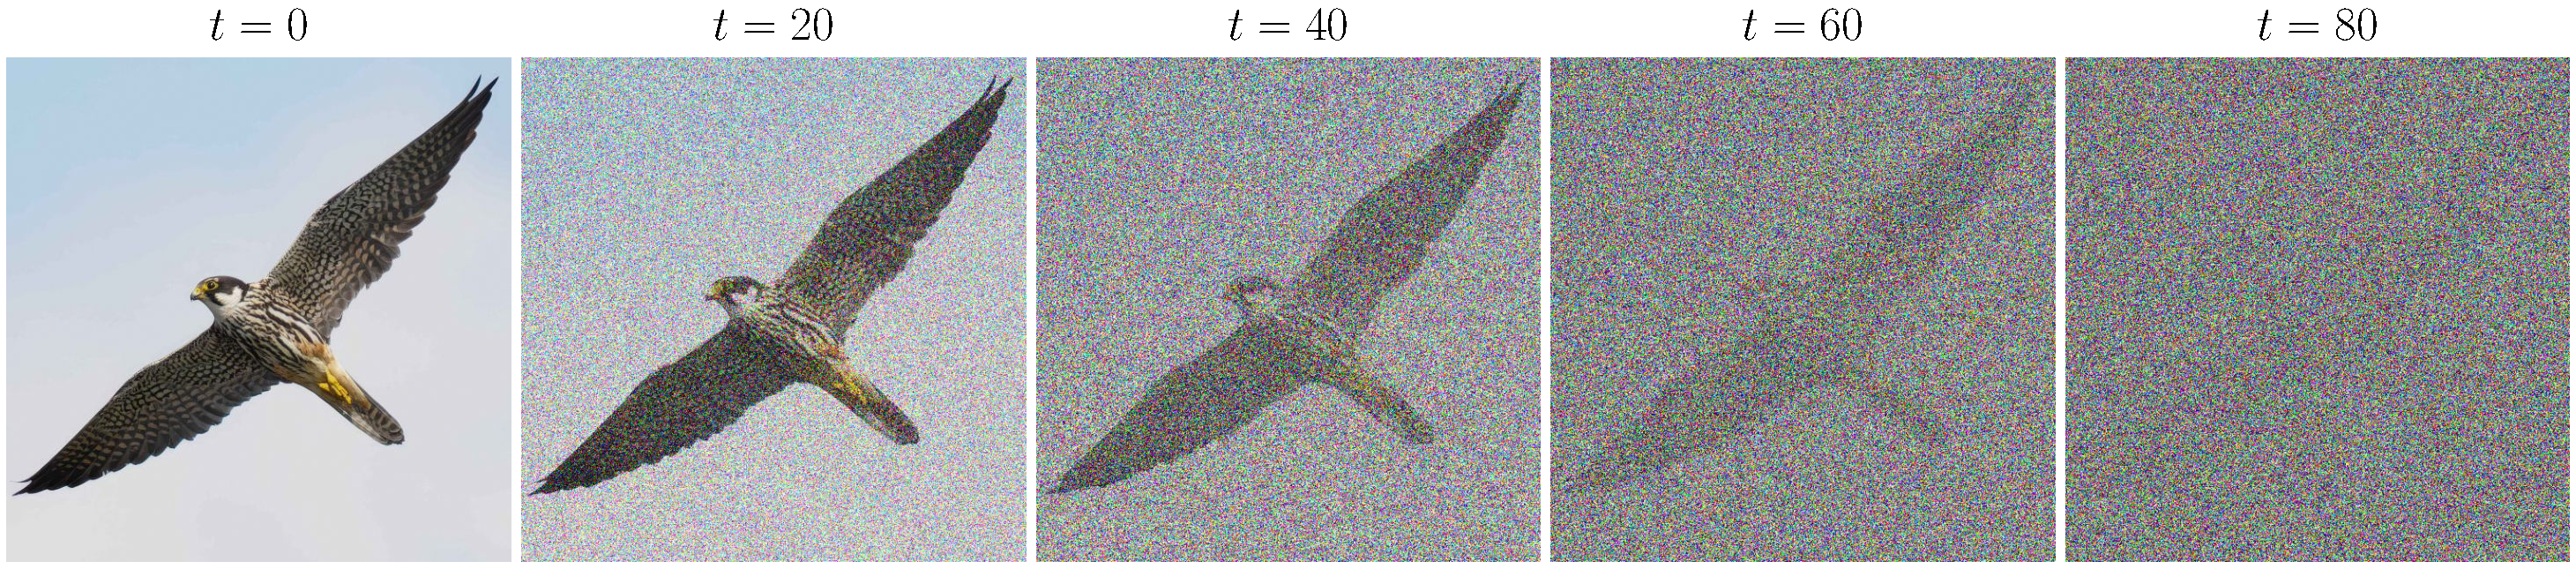
\includegraphics[width=0.85\linewidth]{./Figures/DDPM_Visual.pdf}
		\caption{DDPM\_Visual.pdf}
		\label{Fig_DDPM_Visual}
	\end{figure}
\end{block}
\vspace*{-0.4cm}
\begin{lstlisting}
\begin{figure}[H]
    \centering
    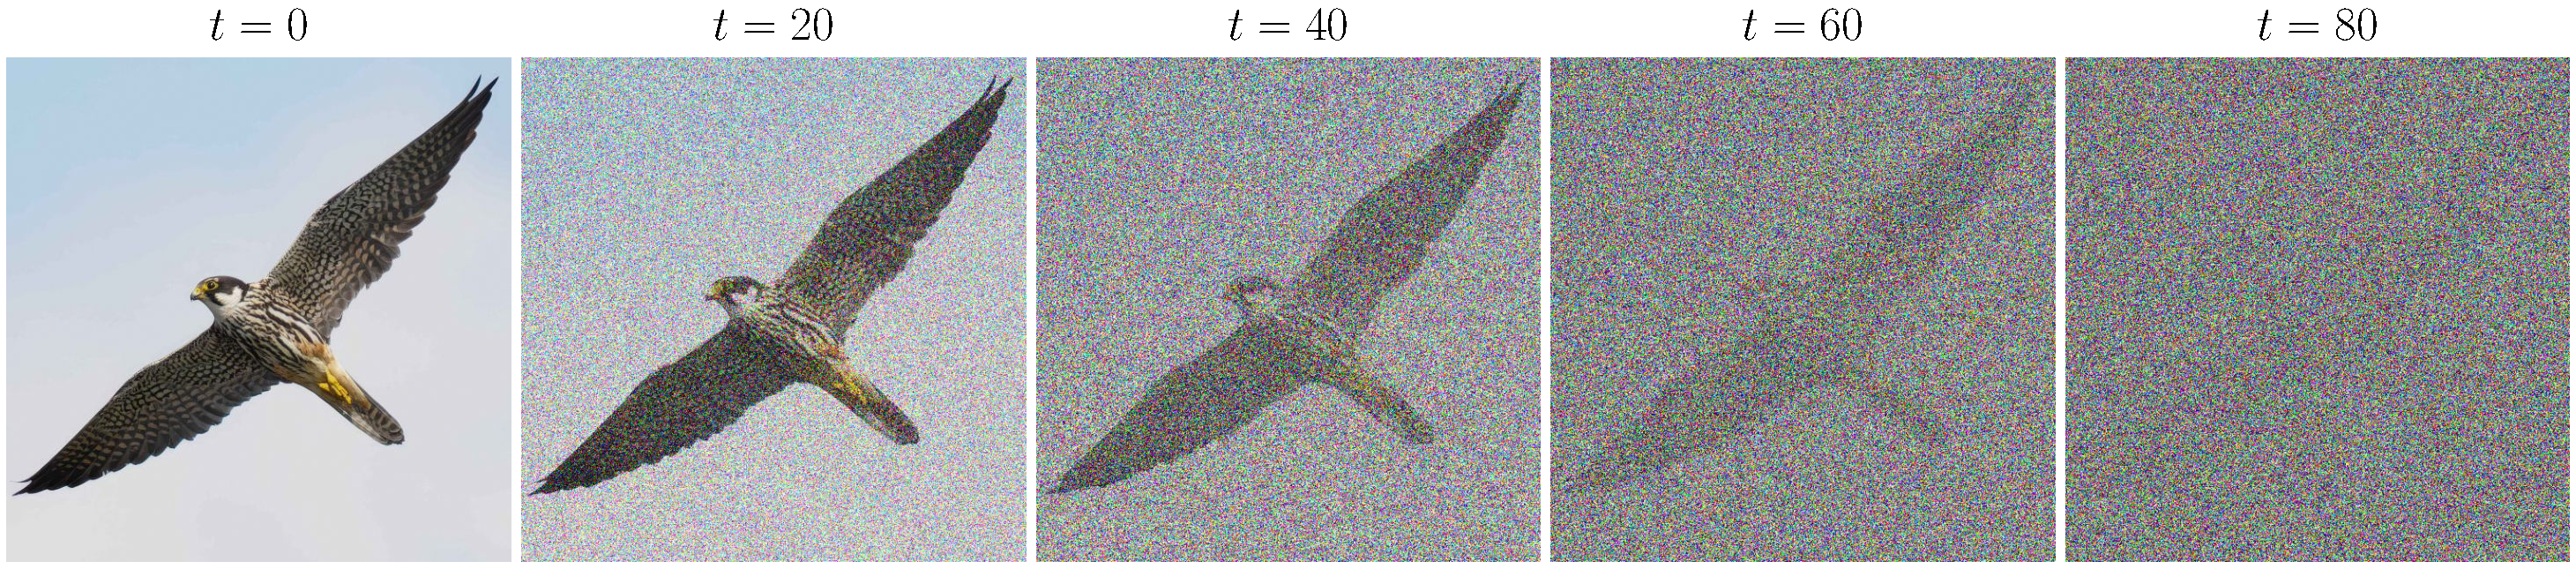
\includegraphics[width=0.3\linewidth]{./Figures/DDPM_Visual.pdf}
    \caption{DDPM\_Visual.pdf}
    \label{Fig_DDPM_Visual}
\end{figure}
\end{lstlisting}

\begin{block}{多子图}
	\begin{figure}[H]
		\centering
		\subfloat[Fig1.png]{
			
\includegraphics[width=0.18\linewidth]{./Figures/Fig1.png}
		}
		\subfloat[Fig2.png]{
			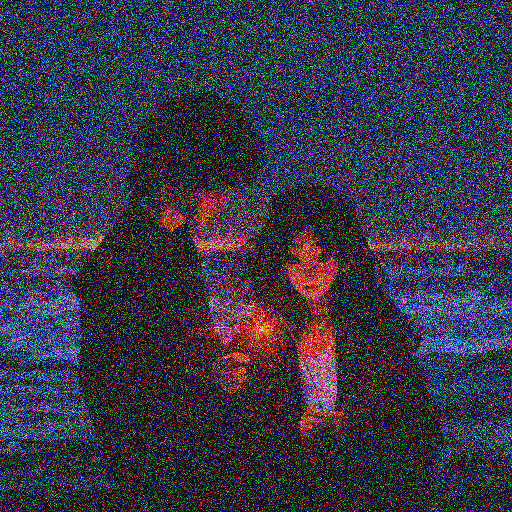
\includegraphics[width=0.18\linewidth]{./Figures/Fig2.png}
		}
		\caption{Fig1.png \& Fig2.png}
		\label{Fig_subfloat}
	\end{figure}
\end{block}
\vspace*{-0.7cm}
\begin{lstlisting}
\begin{figure}[H]
    \centering
    \subfloat[Fig1.png]{
\includegraphics[width=0.2\linewidth]{./Figures/Fig1.png}}
    \subfloat[Fig2.png]{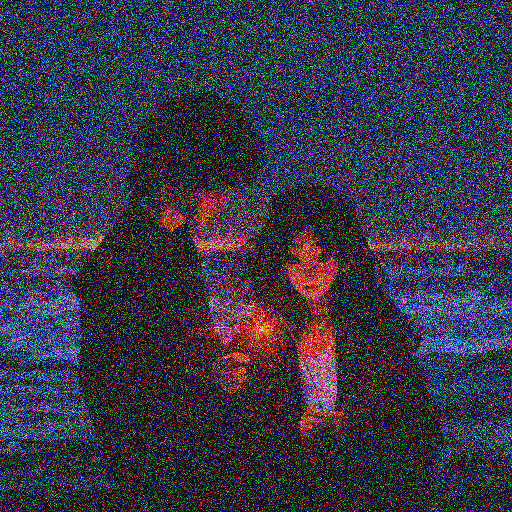
\includegraphics[width=0.2\linewidth]{./Figures/Fig2.png}}
    \caption{Fig1.png \& Fig2.png}
    \label{Fig_subfloat}
\end{figure}
\end{lstlisting}
\end{frame}


\begin{frame}[fragile,allowframebreaks]{表格}
	\begin{block}{表格}
		\begin{table}[H]
			\centering
			\caption{Table Name}
			\label{Table_PSNRandSSIM}
			\footnotesize
			\begin{tabular}{c|c|c||c|c|c}
				\toprule[1.5pt]
				\multirow{2}{*}{\makecell{噪声水平 \\ PSNR / SSIM}} & \multicolumn{2}{c||}{ImageNet32} & \multirow{2}{*}{\makecell{噪声水平 \\ PSNR / SSIM}} & \multicolumn{2}{c}{BSD68} \\
				& 模型名称  & PSNR / SSIM && 模型名称  & PSNR / SSIM \\
				\midrule[0.75pt]\midrule[0.5pt]
				% sigma = 5
				\multirow{5}{*}{\makecell{$\sigma=5$ \\ 34.16 / 0.94}} & BM3D\textsuperscript{\cite{Hunheyu}} & 29.98 / 0.92 & \multirow{5}{*}{\makecell{$\sigma=5$ \\ 39.38 / 0.98}} & BM3D\textsuperscript{\cite{Hunheyu}} & 29.98 / 0.90 \\
				& Shrinkage\textsuperscript{\cite{2014Shrinkage}} & 30.50 / 0.92 && Shrinkage\textsuperscript{\cite{2014Shrinkage}} & 29.11 / 0.90 \\
				& CBDNet\textsuperscript{\cite{2019CBDNet}}          & 37.06 / 0.97 && CBDNet\textsuperscript{\cite{2019CBDNet}}         & 40.07 / 0.98 \\
				& DRANet\textsuperscript{\cite{2024DRANet}}         & 40.55 / 0.99 && DRANet\textsuperscript{\cite{2024DRANet}}          & 40.28 / 0.99 \\
				& \cellcolor[HTML]{EFEFEF}Ours & \cellcolor[HTML]{EFEFEF}38.39 / 0.95 && \cellcolor[HTML]{EFEFEF}Ours & \cellcolor[HTML]{EFEFEF}35.73 / 0.96 \\
				% sigma = 10
				\midrule[0.5pt]\midrule[0.5pt]
				\multirow{5}{*}{\makecell{$\sigma=10$ \\ 28.25 / 0.83}} & BM3D\textsuperscript{\cite{Hunheyu}} & 28.57 / 0.90 & \multirow{5}{*}{\makecell{$\sigma=10$ \\ 33.65 / 0.94}} & BM3D\textsuperscript{\cite{Hunheyu}} & 27.63 / 0.88 \\
				& Shrinkage\textsuperscript{\cite{2014Shrinkage}} & 30.31 / 0.92 && Shrinkage\textsuperscript{\cite{2014Shrinkage}} & 29.03 / 0.90 \\
				& CBDNet\textsuperscript{\cite{2019CBDNet} }         & 32.70 / 0.95 && CBDNet\textsuperscript{\cite{2019CBDNet}}         & 36.46 / 0.97 \\
				& DRANet\textsuperscript{\cite{2024DRANet}}          & 37.05 / 0.98 && DRANet\textsuperscript{\cite{2024DRANet}}         & 36.26 / 0.97 \\
				& \cellcolor[HTML]{EFEFEF}Ours & \cellcolor[HTML]{EFEFEF}36.75 / 0.92 && \cellcolor[HTML]{EFEFEF}Ours & \cellcolor[HTML]{EFEFEF}34.82 / 0.95 \\
				\midrule[0.5pt]\bottomrule[1.5pt]
			\end{tabular}
		\end{table}
	\end{block}
	
	
	\qquad（续表 \ref{Table_PSNRandSSIM}）
	\begin{table}[H]
		\centering
		\footnotesize
		\begin{tabular}{c|c|c||c|c|c}
			\toprule[1.5pt]
			\multirow{2}{*}{\makecell{噪声水平 \\ PSNR / SSIM}} & \multicolumn{2}{c||}{ImageNet32} & \multirow{2}{*}{\makecell{噪声水平 \\ PSNR / SSIM}} & \multicolumn{2}{c}{BSD68} \\
			& 模型名称  & PSNR / SSIM && 模型名称  & PSNR / SSIM \\
			\midrule[0.75pt]\midrule[0.5pt]
			% sigma = 15
			\multirow{5}{*}{\makecell{$\sigma=15$ \\ 24.82 / 0.73}} & BM3D\textsuperscript{\cite{Hunheyu}} & 27.69 / 0.89 & \multirow{5}{*}{\makecell{$\sigma=15$ \\ 30.21 / 0.89}} & BM3D\textsuperscript{\cite{Hunheyu}} & 26.77 / 0.85 \\
			& Shrinkage\textsuperscript{\cite{2014Shrinkage}} & 29.96 / 0.91 && Shrinkage\textsuperscript{\cite{2014Shrinkage}} & 28.88 / 0.89 \\
			& CBDNet\textsuperscript{\cite{2019CBDNet}}          & 29.59 / 0.91 && CBDNet\textsuperscript{\cite{2019CBDNet} }         & 33.78 / 0.96 \\
			& DRANet\textsuperscript{\cite{2024DRANet}}          & 35.08 / 0.97 && DRANet\textsuperscript{\cite{2024DRANet}}         & 34.03 / 0.96 \\
			& \cellcolor[HTML]{EFEFEF}Ours & \cellcolor[HTML]{EFEFEF}34.14 / 0.90 && \cellcolor[HTML]{EFEFEF}Ours & \cellcolor[HTML]{EFEFEF}33.12 / 0.93 \\
			\midrule[0.5pt]\bottomrule[1.5pt]
		\end{tabular}
	\end{table}
	
\begin{lstlisting}
\begin{table}[H]
    \centering
    \caption{Table Name}
    \label{Table_PSNRandSSIM}
    \footnotesize
    \begin{tabular}{表格对齐设置}
        % 表格内容
    \end{tabular}
\end{table}
\end{lstlisting}
\end{frame}


\begin{frame}[fragile,allowframebreaks]{算法流程}
	\begin{center}
		\small
		\begin{minipage}{0.75\linewidth}
			\begin{algorithm}[H]
				% 标题
				\caption{残差噪声扩散模型的推理过程}\label{Resfusion_algorithm_inference}
				\KwIn{
					待恢复退化图像 $\hat{\xb}_0$.
				}
				\KwOut{恢复图像 $\xb_0$.}
				从 $\xb_{T'} \sim \N(\xb_{T'};(1-\sqrt{\bar{\alpha}_{T'}})\hat{\xb}_0,(1-\bar{\alpha}_{T'})\Ib)$ 中抽样 $\xb_{T'}$ \;
				
				\For{$t=T',T'-1,\dots,1$}{
					\eIf{$t>1$}{
						从高斯正态分布 $\zb \sim \N(\zb;\zeros,\Ib)$ 中抽样 $\zb$ \;
					}{
						$\zb=\zeros$ \;
					}
					计算 $\sigma_q(t) = \sqrt{\dfrac{(1-\alpha_t)(1-\bar{\alpha}_{t-1})}{1-\bar{\alpha}_t}}$ \;
					
					计算
					\[
					\xb_{t-1} = \dfrac{1}{\sqrt{\alpha_t}}\left(\xb_t-\dfrac{1-\alpha_t}{\sqrt{1-\bar{\alpha}_t}}res\epsilonb_{\thetab}(\xb_t,\hat{\xb}_{0},t)\right) + \sigma_q(t)\zb
					\]
				}
			\end{algorithm}
		\end{minipage}
	\end{center}
\begin{lstlisting}
\begin{center}
\small
\begin{minipage}{0.75\linewidth}
    \begin{algorithm}[H]
        % 算法内容
    \end{algorithm}
\end{minipage}
\end{center}
\end{lstlisting}
	\vspace*{0.5cm}
	\begin{block}{Tips}
		强烈建议使用 \texttt{minipage} 环境包裹 \texttt{algorithm} 环境，方便控制算法流程的整体宽度。
	\end{block}
\end{frame}



	\section{数学样式}
%\sepframe[image={
\includegraphics[width=3.38cm]{./Figures/Logos/USTC_logo_blue.pdf}}]
% \sepframe 无插入 logo 的分隔页
\sepframe[image={
\includegraphics[width=3.38cm]{./Figures/Logos/USTC_logo_blue.pdf}}]

\begin{frame}[fragile]{自定义数学命令}
	\begin{block}{自定义符号}
	\texttt{Configure/commands.tex} 中定义了常用数学符号，例如
	\[
	\xb,\quad \Rb,\quad \zb,\quad \thetab,\quad \N,\quad \E,\quad \KL,\quad \norm{\xb}_2
	\]
	\end{block}
	
	\begin{block}{示例公式}
		\begin{equation}
			\xb_t=\sqrt{\bar{\alpha}_t}\xb_0+(1-\sqrt{\bar{\alpha}_t})\Rb+\sqrt{1-\bar{\alpha}_t}\epsilonb
			\label{eq_label}
		\end{equation}
		公式引用效果：\eqref{eq_label}。
	\end{block}
\begin{lstlisting}
\begin{equation}
    % 公式内容
    \label{eq_label}
\end{equation}
公式引用效果：\eqref{eq_label}。
\end{lstlisting}
\end{frame}

\begin{frame}{数学样式测试页说明}
	\begin{information}[完整展示]
		\texttt{main.tex} 中的 \texttt{Sections/MathStyleTest.tex} 是自定义数学样式的完整测试页。手册后续会直接导入该文件，因此 \texttt{USTC\_Amurmaple-doc.pdf} 中会完整展示 Definition、Property、Question、Solution、Remark、Example、Theorem、Corollary、Lemma、Proposition 和 Proof 的样式及引用效果。
	\end{information}
	
	\begin{remark}[维护方式]
		只需要修改 \texttt{Configure/beamerMathStyle.tex} 和 \texttt{Sections/MathStyleTest.tex}，重新编译后会同步展示最新数学盒样式。
	\end{remark}
\end{frame}

	\section{扩展命令与编译}
%\sepframe[image={
\includegraphics[width=3.38cm]{./Figures/Logos/USTC_logo_blue.pdf}}]
% \sepframe 无插入 logo 的分隔页
\sepframe[image={
\includegraphics[width=3.38cm]{./Figures/Logos/USTC_logo_blue.pdf}}]

\begin{frame}[fragile]{页内小标题与强调}
	\framesection{页内小标题}
	\texttt{\textbackslash framesection\{...\}} 可在同一页中插入带主题色横线的小标题。
	
	\framesection{盒装强调}
	\texttt{\textbackslash boxalert\{...\}}，例如：\boxalert{这是一个重点结论}。
	
\begin{lstlisting}
\framesection{页内小标题}
\texttt{\textbackslash framesection\{...\}} 可在同一页中插入带主题色横线的小标题。

\framesection{盒装强调}
\texttt{\textbackslash boxalert\{...\}}，例如：\boxalert{这是一个重点结论}。
\end{lstlisting}
\end{frame}

\begin{frame}[fragile]{参考文献、致谢页与编译}
	\begin{block}{参考文献}
		\texttt{Bibliography/Bibliography.tex} 中已经配置好，在正文中使用 \texttt{\textbackslash cite\{\}} 即可得到 [N] 形式。若想修改为 \textsuperscript{[N]} 则使用 \texttt{\textbackslash textsuperscript\{\textbackslash cite\{\}\}}。
	\end{block}
	
	\begin{block}{致谢页}
		\texttt{\textbackslash thanksframe} 用于生成最后的致谢页。可选参数可以替换默认图片；必选参数是致谢文字。
	\end{block}
	
\begin{lstlisting}
\thanksframe{恳请各位老师批评指正！}
\end{lstlisting}

	\begin{block}{推荐编译顺序}
		推荐使用 \hologo{LuaLaTeX}。如果包含参考文献，常见编译顺序为 \texttt{lualatex -> bibtex -> lualatex -> lualatex}。
	\end{block}
\end{frame}

	
	% Bibliography
	% \begin{frame}[fragile, allowframebreaks]{参考文献}
\begin{frame}{参考文献}
	\bibliographystyle{./Bibliography/gbt7714-numerical.bst}
	\footnotesize
	\bibliography{./Bibliography/MyBibliography.bib}
\end{frame}
	
	% Appendix
	\appendix
\section*{附录}
\sepframe[image={
\includegraphics[width=3.38cm]{./Figures/Logos/USTC_logo_blue.pdf}}]
%\sepframe[image={
\includegraphics[width=3.38cm]{./Figures/Logos/USTC_logo_blue.pdf}}]
% \sepframe 无插入 logo 的分隔页
\begin{frame}[fragile]{附录说明与 Beamer Tips}
	\begin{information}[附录说明]
		执行 \texttt{\textbackslash appendix} 后，Amurmaple 主题会将附录部分的页码显示为罗马数字，并且主文档进度条不再继续推进。
	\end{information}
	
	\begin{block}{Beamer Tips}
		\begin{itemize}
			\item 文字缩进可以使用 \texttt{\textbackslash qquad} 手动调整；
			\item 图表排版的大小设置需要手动调整；
			\item \texttt{\textbackslash begin \{minipage\}[]\{\}...\textbackslash end\{minipage\}} 可以用于个性化布局排版，例如竖排图和文字（$1\times2$、$2\times1$ 等布局）。
			\item \texttt{\textbackslash footnote} 脚注命令在 \texttt{minipage} 中与 \texttt{frame} 不关联，此时需要先在 \texttt{minipage} 中使用 \texttt{\textbackslash footnotemark}，然后在 \texttt{frame} 中使用 \texttt{\textbackslash footnotetext} 即可。
			\item 如果需要使用 \texttt{lstlisting} 环境，需要在所处的 \texttt{frame} 环境参数添加 \texttt{fragile}。
			\item 局部布局微调用 \texttt{\textbackslash vspace\textsuperscript{*}\{\}} 和 \texttt{\textbackslash hspace\textsuperscript{*}\{\}} 上下调整和左右调整。
		\end{itemize}
	\end{block}
	
\end{frame}


	
	% MathStyle 测试
	
\begin{frame}[fragile, allowframebreaks]{\texttt{Sections/MathStyleTest.tex}}

	\begin{beamerdefinition}{定义}{dfnref}
		上述实验表明，本文使用的模型不仅能够有效地去除噪声还能够保持和恢复图像的细节，同时对其他的图像恢复任务能适用。上述实验表明，本文使用的模型不仅能够有效地去除噪声还能够保持和恢复图像的细节，同时对其他的图像恢复任务能适用。
	\end{beamerdefinition}
	关于 Definition \ref{dfn:dfnref} 的引用.
	
	
	\begin{beamerproperty}{性质}{proref}
		上述实验表明，本文使用的模型不仅能够有效地去除噪声还能够保持和恢复图像的细节，同时对其他的图像恢复任务能适用。上述实验表明，本文使用的模型不仅能够有效地去除噪声还能够保持和恢复图像的细节，同时对其他的图像恢复任务能适用。
	\end{beamerproperty}
	关于 Property \ref{pro:proref} 的引用.
	
	\begin{beamerquestion}{某次课的问题}{qsref}
		上述实验表明，本文使用的模型不仅能够有效地去除噪声还能够保持和恢复图像的细节，同时对其他的图像恢复任务能适用。上述实验表明，本文使用的模型不仅能够有效地去除噪声还能够保持和恢复图像的细节，同时对其他的图像恢复任务能适用。
	\end{beamerquestion}
	关于 Question \ref{qs:qsref} 的引用.
	
	\beamersolution{解答开始...}
	
	
	\begin{beamerremark}{注意}{rmkref}
		上述实验表明，本文使用的模型不仅能够有效地去除噪声还能够保持和恢复图像的细节，同时对其他的图像恢复任务能适用。上述实验表明，本文使用的模型不仅能够有效地去除噪声还能够保持和恢复图像的细节，同时对其他的图像恢复任务能适用。
	\end{beamerremark}
	关于 Remark \ref{rmk:rmkref} 的引用.
	
	
	
	\begin{beamerexample}{一个例子}{exref}
		上述实验表明，本文使用的模型不仅能够有效地去除噪声还能够保持和恢复图像的细节，同时对其他的图像恢复任务能适用。上述实验表明，本文使用的模型不仅能够有效地去除噪声还能够保持和恢复图像的细节，同时对其他的图像恢复任务能适用。
	\end{beamerexample}
	关于 Example \ref{ex:exref} 的引用.
	
	
	
	\begin{beamertheorem}{高斯定理}{thmref}
		上述实验表明，本文使用的模型不仅能够有效地去除噪声还能够保持和恢复图像的细节，同时对其他的图像恢复任务能适用。上述实验表明，本文使用的模型不仅能够有效地去除噪声还能够保持和恢复图像的细节，同时对其他的图像恢复任务能适用。
	\end{beamertheorem}
	关于 Theorem \ref{thm:thmref} 的引用.
	

	\begin{beamercorollary}{高斯定理的推论}{corref}
		上述实验表明，本文使用的模型不仅能够有效地去除噪声还能够保持和恢复图像的细节，同时对其他的图像恢复任务能适用。上述实验表明，本文使用的模型不仅能够有效地去除噪声还能够保持和恢复图像的细节，同时对其他的图像恢复任务能适用。
	\end{beamercorollary}
	关于 Corollary \ref{cor:corref} 的引用.
	
	\begin{beamerlemma}{费马引理}{lmref}
		上述实验表明，本文使用的模型不仅能够有效地去除噪声还能够保持和恢复图像的细节，同时对其他的图像恢复任务能适用。上述实验表明，本文使用的模型不仅能够有效地去除噪声还能够保持和恢复图像的细节，同时对其他的图像恢复任务能适用。
	\end{beamerlemma}
	关于 Lemma \ref{lm:lmref} 的引用.
	
	\begin{beamerproposition}{简单命题}{prpref}
		上述实验表明，本文使用的模型不仅能够有效地去除噪声还能够保持和恢复图像的细节，同时对其他的图像恢复任务能适用。上述实验表明，本文使用的模型不仅能够有效地去除噪声还能够保持和恢复图像的细节，同时对其他的图像恢复任务能适用。
	\end{beamerproposition}
	关于 Proposition \ref{prp:prpref} 的引用.
	
	\begin{proof}
		随便证明点东西吧。上述实验表明，本文使用的模型不仅能够有效地去除噪声还能够保持和恢复图像的细节，同时对其他的图像恢复任务能适用。
	\end{proof}
	
	\vspace*{1cm}
	\boxalert{MathStyleTest 的用法直接查看 \texttt{Sections/MathStyleTest.tex} 源文件即可。}
\end{frame}
	
	% Thanksframe
	\thanksframe{感谢 Beamer Amurmaple 主题的所有开源项目！}
\end{document}
